\chapter{Blockchain technology} \label{chap:Blockchain}

As identified in the introduction, this technology is difficult for many to understand as it lies at the intersection of cryptography, game theory, computer networking, data transmission and monetary theory.\footcite[Cf.][]{LoppNobodyUnderstandsBitcoin2017} The different concepts interact very closely and thus multiple elements must be understood concurrently.\footcite[Cf.][p.2]{SwellerVisualisationInstructionalDesign2002} This chapter gives a  brief introduction to the technology. It provides an overview of the motivation behind its creation \& the general elements of a blockchain and subsequently examines transactions and their broadcast as well as possible applications. 
% Wieso ist Blockchain für viele so schwer zu verstehen? -> Intersection of different topics -> Information Structures (Sweller 1994)

\section{An overview of the blockchain} \label{sec:Blockchain}

Blockchain technology was first introduced in the wake of the global economic crisis, in 2008, when a person under the pen name Satoshi Nakamoto presented a concept for a new digital currency.\footcite[Cf.][]{Nakamoto.2008} With the motivation to provide a financial system without relying on banks or other financial institutions as intermediaries, they introduced the digital currency Bitcoin. In his paper, Nakamoto criticizes the central role of the financial institution controlling digital transactions between two parties and forcing these two parties to trust the institution. Instead of using the service of such a central institution, which could possibly tamper with the transaction if it were compromised or ceded executing any transaction in the case of a downtime, he develops a system allowing any two parties to conduct transactions directly with each other, thus removing the need for a trusted third party.\footcite[Cf.][p.2]{Nakamoto.2008} A blockchain can be thought of as a decentralised ledger which records the entire transaction\footnote{A transaction refers to one change made in the ledger. E.g. Payment of one bitcoin from A to B} history. The name stems from the fact that transactions are bundled into blocks. Each block in the blockchain (except for the first i.e. genesis block) references a previous block.\footcite[Cf.][chapter 1]{BashirMasteringBlockchain2017} By connecting the blocks in this manner, all changes in the ledger can be reconstructed and all transactions are at all times visible. It runs on a peer-to-peer network of computers provided by volunteers around the world and without a central database to possibly hack or shut down. Each node participating in the network has its own copy of the blockchain, hence giving all nodes the same view of the blockchain.\footcites[Cf.][p.5]{Tapscott.2017}[cf.][p.41]{Welzel.2017} Its distributed nature allows the system to stay healthy even if some nodes quit the network or are compromised. This approach protects the blockchain against possible power outages or unilateral manipulation.\footcite[Cf.][p.8]{Nakamoto.2008}

To establish a consensus between the nodes agreeing on which transactions are valid and can be included in the blocks, the participating nodes first verify the validity of every new transaction by cryptographically verifying that the initiating party actually owns the coins it is sending to the receiving party and that they have not been spent on something else.\footcite[cf.][p.68]{AntonopolousAndreasM..2017} Then, the nodes participate in a distributed consensus mechanism to build the next block that is then appended to the blockchain. In the case of Bitcoin, this takes place on the basis of the Proof of Work algorithm.\footcites[Cf.][]{Dwork.1993}[cf.][p.3]{Nakamoto.2008} Proof of Work takes advantage of a cryptographic puzzle, where a node has to use its computing resources in order to find a random number, called nonce (number used only once), so that the hash of the signature of the previous block, the transactions of the current block, a time stamp, and said nonce results in a value that has a specific set of leading zeroes. The cryptographic puzzle is secure against cheating because two similar values result in two totally different and random hashed values. It is not possible with today's tools to calculate the original value from a hashed value. This cryptographic puzzle therefore forces the node to use its CPU capacity to find a random nonce. Only with such a nonce will a new block broadcast to the network be accepted by the other nodes.\footcites[Cf.][p.8]{Nakamoto.2008}[cf.][p.12]{Schutte.2017} Apart from the CPU based Proof of Work algorithm, there are a number of other distributed consensus mechanisms. For example, the Proof of Work approach has been adapted to a memory based algorithm where the puzzle has to be solved by a specific number of memory reads.\footcite[Cf.][]{Abadi.2005} It has also been adapted to a network-based approach where the puzzle is solved by communicating with other nodes on the network and using their information to complete the puzzle.\footcite[Cf.][]{Abliz.2009} Another approach is Proof of Stake as implemented by another blockchain Ethereum. In this approach, the nodes that can build a new block are chosen from their share of their digital currency\footcite[Cf.][]{King.2012} or they are chosen randomly.\footcites[Cf.][]{w.A..2016}[cf.][p.200]{AntonopolousAndreasM..2017}[cf.][p.11-12]{Schlatt.2016}

Independently of its consensus mechanism, a blockchain can take different forms:\footcite[Cf.][p.10-12]{Schlatt.2016}
\begin{itemize}
  \item \textbf{Public Blockchain:} The ledger is public and everyone can join the network.
  \item \textbf{Private Blockchain:} The ledger is accessible to a predefined set of users.
  \item \textbf{Permissionless Blockchain:} All nodes in the network are equal and all can append to the blockchain.
 \item \textbf{Permissioned Blockchain:} A predefined subset of nodes in the network has the right to append to the blockchain. All nodes broadcast their transactions to the network but only the permissioned nodes create new blocks.
\end{itemize} 

\begin{figure}[h!]
 \centering
 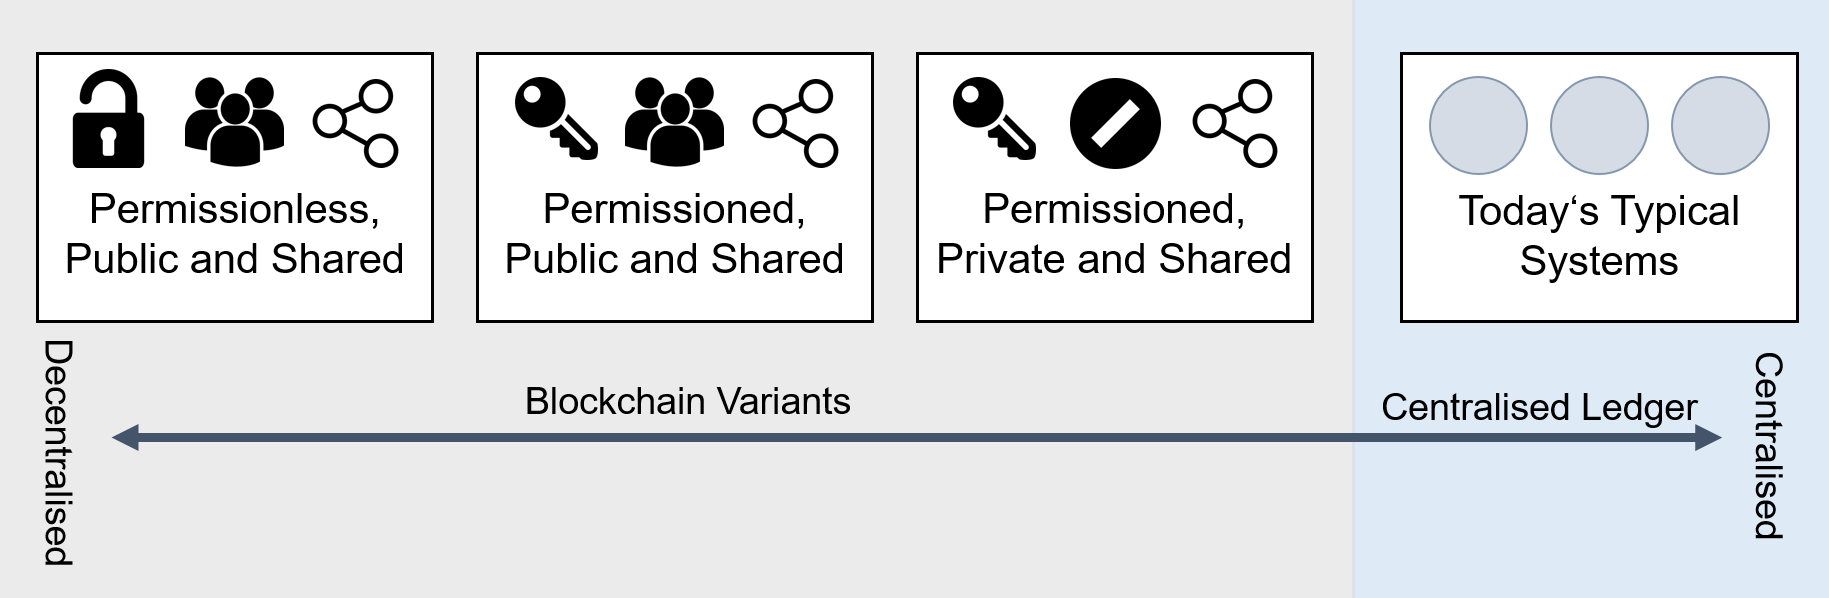
\includegraphics[width = \textwidth]{graphics/Picture1.png}
 \caption{Different blockchains vary in their degree of centralization, adapted from \cite{GOV.2016}.}
 \label{fig:DLTs}
\end{figure}

The capabilities of blockchain go far beyond providing a distributed ledger if smart contracts are used. Smart contracts are pieces of code in a transaction which are executed when nodes validate that transaction. These smart contracts extend the capabilities of blockchain to allow trusted and automatic modification of information.\footcite[Cf.][p.14]{Schutte.2017} They are in their essence a digital copy of a conventional contract, defining the rules and punishments in the case of non-compliance in lines of code. The concept of describing a contract with code was introduced in 1997 by Nick Szabo\footcite[][]{Szabo.1997} but only in combination with blockchain can it be implemented to develop its full effect.\footcites[Cf.][p.23]{Schlatt.2016}[cf.][p.22-24]{GOV.2016} Processes, which validate the integrity of an entity, may be fully automated by using blockchain technology and smart contracts.

In conclusion, blockchain technology shows the following characteristics: It is distributed, digital transactions no longer necessitate a middleman to be executed securely. The blockchain is encrypted, it uses public and private key pairs to establish virtual security. Blockchain is also for the most part public, anyone is able to view all transactions at all times because they lie on the network and not in one central database, and the code is open-sourced. Finally, the technology enables an immutable, complete history of all transactions.\footcite[Cf.][p.5]{Tapscott.2017} All these characteristics combined constitute blockchain's potential to disrupt economic sectors as well as social constructs by eliminating the need of a trusted third party. 

\section{Transactions} \label{sec:TX}

Inspect transactions in detail, show how they are broadcast and put into blocks
-> only in ethereum or bitcoin or should I inspect the overall design of transaction by looking at different coins?

Even though the first implementation of blockchain was motivated by providing a decentralized alternative to financial institutions,\footcite[Cf.][p.2]{Nakamoto.2008} the new defined data structure offers a variety of additional use cases that will be explored in the following section.

\section{Applications of blockchain technology} \label{sec:SmartContracts}

-> here also, only on ethereum or also others? What about legally binding smart contracts?




\section{An overview of the blockchain}
A very brief definition of the blockchain is : ... It was first implemented by Satoshi Nakamoto in the form of Bitcoin, a virtual currency with the objective of replacing central financial institutions.

The technology lies at the intersection of the following concepts, which are briefly explained in the following paragraphs:

\paragraph{Networking}
\paragraph{Cryptography}
\paragraph{Monetary theory}
\paragraph{Game theory}
